
\documentclass[a4paper]{easychair}
\usepackage{doc}
\usepackage{enumitem}
% use this if you have a long article and want to create an index
% \usepackage{makeidx}

% In order to save space or manage large tables or figures in a
% landcape-like text, you can use the rotating and pdflscape
% packages. Uncomment the desired from the below.
%
% \usepackage{rotating}
% \usepackage{pdflscape}

% Some of our commands for this guide.
%

%\makeindex

%% Front Matter
%%
% Regular title as in the article class.
%
\title{Automatic covariates selection in dynamic regression models with application to COVID-19 evolution}
% \thanks{Other people who contributed to this document include Maria Voronkov
%   (Imperial College and EasyChair) and Graham Gough (The University of
%   Manchester).}

% Authors are joined by \and. Their affiliations are given by \inst, which indexes
% into the list defined using \institute
%
\author{
    Ana X. Ezquerro \inst{1}
\and
    Germán Aneiros \inst{2}
\and
   Manuel Oviedo de la Fuente \inst{3}
}

% Institutes for affiliations are also joined by \and,
\institute{
   University of A Coruña, \texttt{ana.ezquerro@udc.es}
\and
    Grupo MODES, Departamento de Matemáticas, University of A Coruña, CITIC \\ \texttt{german.aneiros@udc.es}
\and
Grupo MODES, Departamento de Matemáticas, University of A Coruña, CITIC \\ \texttt{manuel.oviedo@udc.es}
}
\authorrunning{Ana X. Ezquerro, Germán Aneiros-Pérez, Manuel Oviedo}

%  \authorrunning{} has to be set for the shorter version of the authors' names;
% otherwise a warning will be rendered in the running heads. When processed by
% EasyChair, this command is mandatory: a document without \authorrunning
% will be rejected by EasyChair

% \authorrunning{Mokhov, Sutcliffe and Voronkov}

% \titlerunning{} has to be set to either the main title or its shorter
% version for the running heads. When processed by
% EasyChair, this command is mandatory: a document without \titlerunning
% will be rejected by EasyChair
\titlerunning{XoveTIC Proceedings 2022}

\begin{document}

\maketitle

\begin{abstract}
    This work introduces a new approach in time-series analysis field for automatic covariates selection in dynamic regression models. Based on \cite{cryer2008time} and \cite{hyndman2018forecasting} previous study, a forward-selection method is proposed for adding new significant covariates from a given set. This algorithm has been implemented and optimized in R as a package, and it has been applied to multiple simulations to validate its performance. Finally, the obtained results from the IRAS database of Catalonia are presented to analyze the COVID-19 evolution. 
\end{abstract}

% The table of contents below is added for your convenience. Please do not use
% the table of contents if you are preparing your paper for publication in the
% EPiC Series or Kalpa Publications series

\setcounter{tocdepth}{2}
{\small
\tableofcontents}

\section{Introduction}

In time-series analysis, the well-known dynamic regression models allow formally modelling the dependence between a set of covariates and a dependent variable considering the intrinsic temporal component of all participant variables. Thus, this type of regression models are of widespread application in diverse scenarios where it is required to analyze the effect of recollected data in a time series of interest. 

Formally, dynamic linear regression models define the linear dependence between a stochastic proccess $Y_t$ (the dependent variable) and a set of proccesses  $\mathcal{X}=\{ X_t^{(1)}, X_t^{(2)}, ..., X_t^{(m)}\}$ (candidates for regressor variables) in times non-greater than $t$:

\begin{equation}\label{dynamic.regression.model}
Y_t = \beta_0 + \beta_1 X^{(1)}_{t-r_1} + \beta_2 X^{(2)}_{t-r_2} + \cdots + \beta_m  X^{(m)}_{t-r_m} + \eta_t 
\end{equation}

\noindent where $r_i \geq 0$, for $i=1,...,m$, and $\eta_t \sim$ ARMA(p,q).

% ¿debería añadir aquí alguna referencia a lo que es un ARMA/ARIMA?


In this work we formally introduce a new algorithm to select covariates which significantly influence the behavior of a dependent variable. Due to the impact of COVID-19 around the world, we use this method to formalize and study the relation of the COVID-19 evolution in Catalonia (Spain) with the flu syndrome, COVID-19 vaccination and other recollected variables from the IRAS database.

\section{Methodology}

Following the definition in (\ref{dynamic.regression.model}), \cite{cryer2008time} proposed a method named \textit{prewhitening} for removing spurious correlation (false linear correlation) between two processes $X_t$ and $Y_t$ (where one of them is not white noise and/or the other is not stationary) by analyzing the cross correlation function 

\begin{equation}\label{cross.correlation}
\rho_k(\ddot{X}_t, \ddot{Y}_t) =  \cfrac{\text{Cov}(\ddot{X}_t, \ddot{Y}_{t-k})}{\sigma_{\ddot{X}_t} \sigma_{\ddot{Y}_t}}
\end{equation}

\noindent where $\sigma_{Z_t}$ denotes the standard deviation of a stochastic process $Z_t$ and $\ddot{X}_t$ and $\ddot{Y}_t$ are obtained via some linear filter application to $X_t$ and $Y_t$ ensuring one of them is white noise and the other is a stationary process. Specifically, \cite{cryer2008time} proposes a real linear correlation between $X_t$ and $Y_t$ if exists some $k$ where $\rho_k(X_t, Y_t)$ is statistically significant. This method is applied to obtain the optimal lags of each regressor in (\ref{dynamic.regression.model}), considering the condition of $k$ being less or equal than $0$.

Our approach iteratively adds dependent processes to a model by checking if a significant correlation (analyzing (\ref{cross.correlation}) as in \cite{cryer2008time}) exists between a new proccess (candidate for regressor variable) and the residuals $\eta_t$ of a simpler model.

Let $Y_t$ be the stochastic dependent proccess and $\mathcal{X}$ be the set of processes that might act as regressor variables in the model (candidates), and an information criterion (IC) for model evaluation. Our method proceeds as follows:


\begin{enumerate}
    \item Initialization. Consider the process $\tilde{Y}_t=Y_t$ that will be used to check the existence of linear correlation between $Y_t$ and each $X_t\in \mathcal{X}$ with \cite{cryer2008time} method, $\nu=\infty$ the value of the IC corresponding to the best model with (\ref{dynamic.regression.model}) form, $\mathcal{X}^{(r,s)}$ the set of selected covariates paired with their respective optimal lags and $\mathcal{X}^{(s)}$ the set of selected covariates (with no lag information). Let $\mathcal{M}(\mathcal{Z})$ be the fitted dynamic regression model regarding $Y_t$ where $\mathcal{Z}$ is the set of covariates paired with their optimal lags:
    \[ \mathcal{M}(\mathcal{Z}) := Y_t = \beta_0 + \sum_{(Z_t, r)\in\mathcal{Z}} \beta^{(Z_t, r)} Z_{t-r} + \eta_t\]
    \noindent where $\beta^{(Z_t, r)}$ is obtained via some estimation.

    \item Iterative selection. For each $X_t\in\mathcal{X}-\mathcal{X}^{(s)}$, obtain the optimal lag where the maximum linear cross correlation between $X_t$ and $\tilde{Y}_t$ occurs in (via \cite{cryer2008time} method). Consider the process $X_t^\text{best}\in\mathcal{X}-\mathcal{X}^{(s)}$ that minimizes and improves $\nu$ value, based on the selected IC, by including it in the model with its optimal lag ($r_{X_t^\text{best}}$):
    
    \begin{equation}\label{iterative.selection}
        X^\text{best}_t =  \underset{X_t\in\mathcal{X}-\mathcal{X}^{(s)}}{\arg\min} \Bigg\{ \ \text{criteria}\Bigg(\ \mathcal{M}\Big(\mathcal{X}^{(s,r)} \cup \big\{(X_t, r_{X_t})\big\} \Big) \ \Bigg) \Bigg\}
    \end{equation}

    \noindent conditioned to $\text{criteria}(\cdot) < \nu$\footnote{for simplicity, we denote the expression in $\text{criteria}()$ in (\ref{iterative.selection}) as $\cdot$}. 
    If $X^{\text{best}}_t$ exists, consider $\mathcal{X}^{(s,r)} = \mathcal{X}^{(s)}  \cup \{(X_t^\text{best}, r_{X_t^\text{best}})\}$, $\tilde{Y}_t = \eta_t$ and $\nu=\text{criteria}(\mathcal{X}^{(s)})$\footnote{once $X_t^\text{best}$ has been added to the model }.
    
    Repeat this step until no process $X_t\in\mathcal{X}-\mathcal{X}^{(s)}$ can be added to the model, i.e. $X_t^\text{best}$ does not exist.


    \item Finalization. If the errors $\eta_t$ of $\mathcal{M}(\mathcal{X}^{(s,r)})$ are not stationary and no model with $\eta_t\sim\text{ARMA(p,q)}$ and $\mathcal{X}(s,r)$ covariates can be adjusted, consider the regular differentiation of all data (dependent variable and regressor candidates) and return to (1). Otherwise, it is proven that  $\mathcal{M}(\mathcal{X}^{(s,r)})$ with stationary errors defines the significant correlation between the set of $\mathcal{X}^{(s)}$ regressor variables and the dependent proccess $Y_t$.
\end{enumerate}

This algorithm was implemented in R programming language. The step 2 was optimized by parallelizing the fit of independent models of each candidate in $\mathcal{X}$. \cite{dickey1979distribution} test is used for checking proccesses stationary and \cite{Haynes2013, shapiro1965analysis, Jarque2011, ljungbox1970, ljungbox1978} tests to check the independence, normality and zero mean of ARIMA residuals. 

\section{Simulation results}

In order to validate the performance of our selection method, we simulate multiple scenarios where a time series $Y_t$ was artificially constructed with other variables (introduced with their respective coefficients and lags as in (\ref{dynamic.regression.model})), which were added to a set of candidates along with more variables which do not influence in the construction of $Y_t$. The algorithm was tested when the residuals of the model $\eta_t$ were stationary and non-stationary. 

\section{COVID-19 application}


\begin{figure}
    \centering
    \label{covid19application}
    \caption{Point predictions at forecast horizon $h=10$ for COVID19 evolution}
    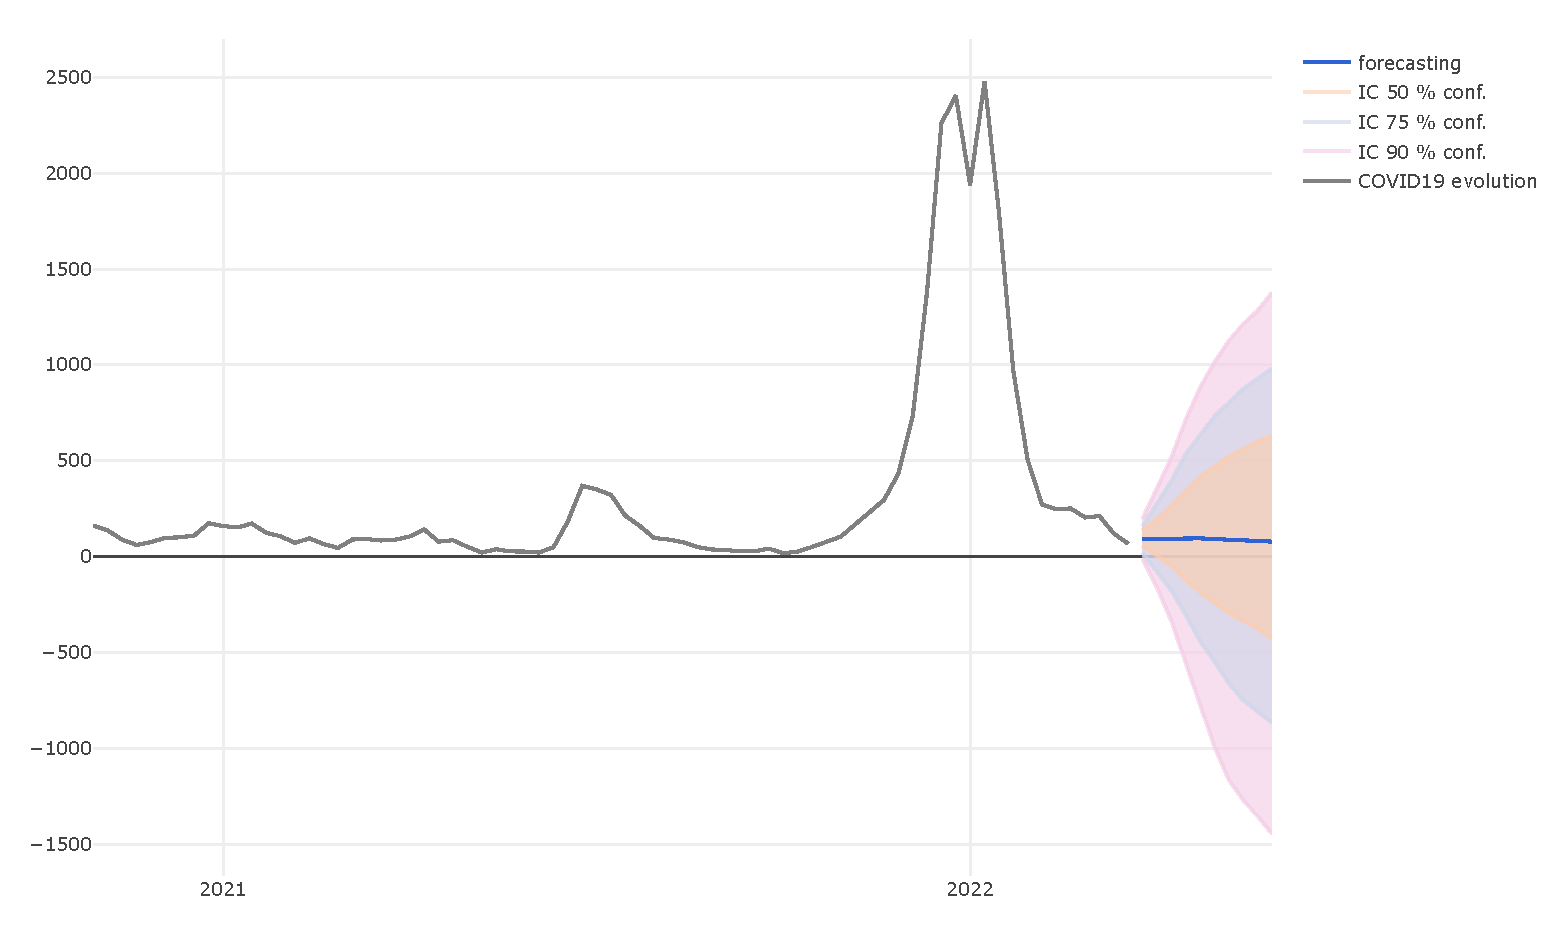
\includegraphics[scale=0.55]{preds_covid19_vac.pdf}
\end{figure}


\begin{table}
    \centering
    \setlength{\tabcolsep}{20pt}
    \label{covid19model}
    \caption{Information about the dynamic regression model constructed via selection of multiple vaccination variables to model COVID19 evolution} 

    \vspace{1em}
    \begin{tabular}{|l|rrr|}
        \hline
        \textbf{Covariate}  & \textbf{Lag}  & \textbf{IC achieved}  & \textbf{Coefficient estimation (s.e)} \\ 
        \hline 
        \texttt{vac1218}    & -6            & 902.564               & -0.0707 (0.0491)                      \\
        \texttt{vac4565}    & -3            & 883.685               & 0.0511 (0.0046)                       \\ 
        \texttt{vac6580}    & -2            & 877.400               & -0.0750 (0.0095)                      \\
        \texttt{vac1845}    & -6            & 869.236               & -0.0559 (0.0211)                      \\
        \hline
        \texttt{vac80}      & \multicolumn{3}{c|}{Not included in the model} \\
        \hline        
    \end{tabular}
\end{table}

Our approach was tested in the IRAS (\textit{acute respiratory infections}) database of Catalonia (Spain) in order to analyze the evolution of COVID-19 and the impact of other variables, such as the vaccination progress and influenza confirmed cases. In addition, individual data was aggregated by age ranges and Health Areas to study the correlation between groups and their influence in the global evolution. 

Figure (\ref{covid19application}) shows puntual predictions based on a fitted dynamic regression model where the COVID19 evolution is linearly defined by the vaccination of different age groups. Table (\ref{covid19model})\footnote{where \texttt{vac1218}, \texttt{vac1845}, \texttt{vac4565}, \texttt{vac6580} denote the vaccination in population from 12, 18, 45 and 65 up to 18, 45, 65 and 80 years (exclusive), respectively, and \texttt{vac80} denotes the vaccination in population from 80 years.} resumes the algorithm trace and the order of covariates addition to the model.

\bibliographystyle{plain}
\bibliography{bibliography}

\end{document}
